\chapter{Coronal Dimming Case Studies}
\label{chaptercasestudy}

% Mini-abstract
This chapter focuses on the detailed analysis of two coronal dimming events. One was selected for its relative simplicity, involving only mass-loss dimming and thermal dimming, while the other was selected for its complexity, involving nearly all of the types of dimming as described in Chapter \ref{chaptermechanisms}. The EUV irradiance and imaging observations of these events as well as the related coronagraph observations are first described in Section \ref{sec:observations}. A new method for deconvolving flare emission from dimming irradiance measurements is developed in Section \ref{sec:deconvolve} while Section \ref{sec:deconvolveerrors} contains the associated error propagation. Finally, Section \ref{sec:casestudyresults} provides analyses and results of these two coronal dimming events. We find that the new deconvolution method for irradiance successfully matches the dimming profile extracted from the spatially-isolated dimming as obtained from EUV image time series. Thus, we show that it is possible to accurately characterize dimming in a localized area even with no spatial resolution. 

\section{Observations}
\label{sec:observations}

\subsection{Simple Dimming Case}
This event occurred on 2010 August 7 at approximately 18:24 UT. The eruptive event consisted of an M1.0 flare, dimming in the region around the flare, and a coronal mass ejection (CME). Other active regions were also on disk but did not have any significant sympathetic responses. Mass-loss and thermal dimming were found to be important, while the other type of dimming (see Chapter \ref{chaptermechanisms}) were negligible. 

\paragraph{Coronagraph Observations}

\begin{figure}[!h]
	\caption[LASCO coronagraph data for 2010 August 7 event]{
        CME event at 19:00 on 2010 August 7. Left: difference image from LASCO C2 and AIA 193 \AA\ channel. 
        Right: CME height versus time shows nearly linear velocity of 871 $km\ s^{-1}$. 
        Figure adapted from CDAW CME Catalog, courtesy of S. Yashiro and N. Gopalswamy.
	}
    \begin{center}
	    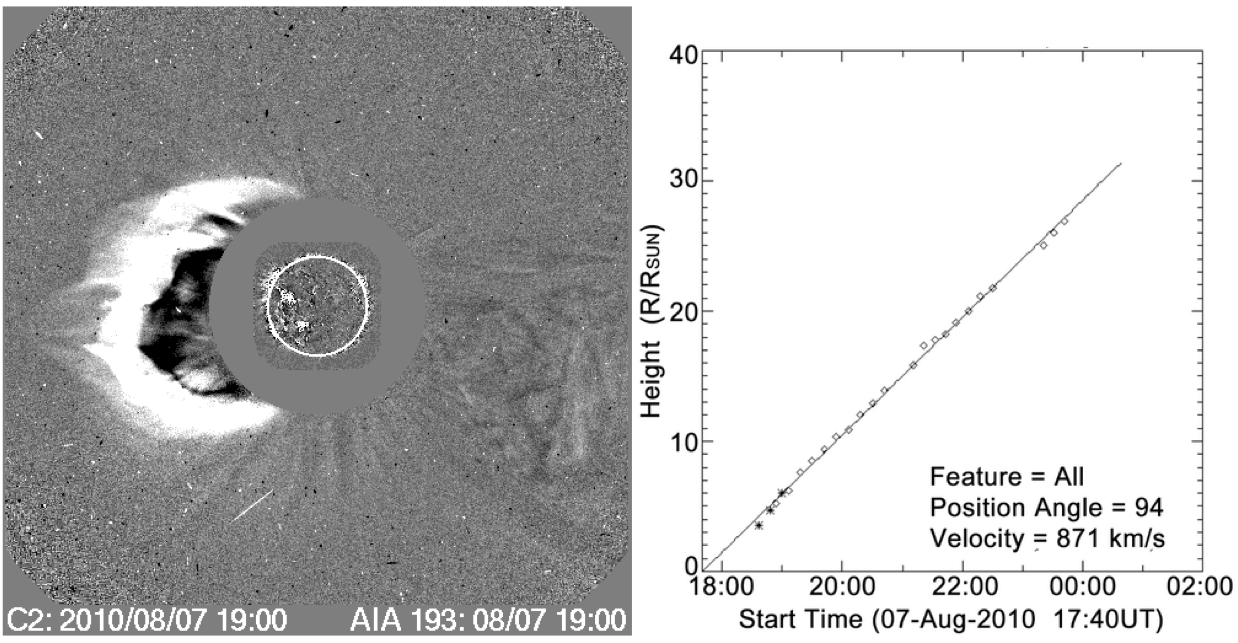
\includegraphics[width=150mm]{Images/Lasco2010Aug7Cme.png}
    \end{center}
    \label{lasco2010aug7}
\end{figure}

The Coordinated Data Analysis Workshops (CDAW) LASCO CME catalog (herein referred to simply as the CDAW catalog) is an extensive database of all CMEs observed by the SOHO/LASCO coronagraphs with related quantities such as date, time, computed velocity, and sometimes mass \citep{Gopalswamy2009}. The CDAW catalog has seven CME events listed for 2010 August 7. All but two of them occur prior to the M1.0 flare at 18:24 UT that is of primary interest for the present study. The CME shown in Figure \ref{lasco2010aug7} is flagged as a halo event with a time of 18:36 UT in CDAW, while the next event occurred with a central position angle of 116\degree\ at 22:24 UT. The timing and location of the flare and associated dimming region suggest that the halo CME is associated with the dimming. The plane-of-sky velocity estimate for this CME is 871 $km\ s^{-1}$ as indicated in Figure \ref{lasco2010aug7}. No mass is listed for this CME in CDAW, but using LASCO and STEREO data and the techniques outlined in \citet{Colaninno2009}, a mass of $6.4 \times 10^{15}$ g was computed for this CME event (A. Vourlidas 2014, private communication). A true space velocity was also computed as 850 $km\ s^{-1}$ at 9 R\astrosun\ with a deceleration of 6.84 $m\ s^{-2}$ (Figure \ref{stereo2010aug7}). Based on these estimates for mass and velocity, this CME is
considered be of modest size.

\begin{figure}[!h]
	\caption[LASCO coronagraph data for 2010 August 7 event]{
        Left: STEREO -A COR2 image at 19:24 UT. Right: CME height vs. time calculated from STEREO and shows a deceleration
        of 6.84 $m\ s^{-2}$. Figure courtesy of Barbara Thompson. 
	}
    \begin{center}
	    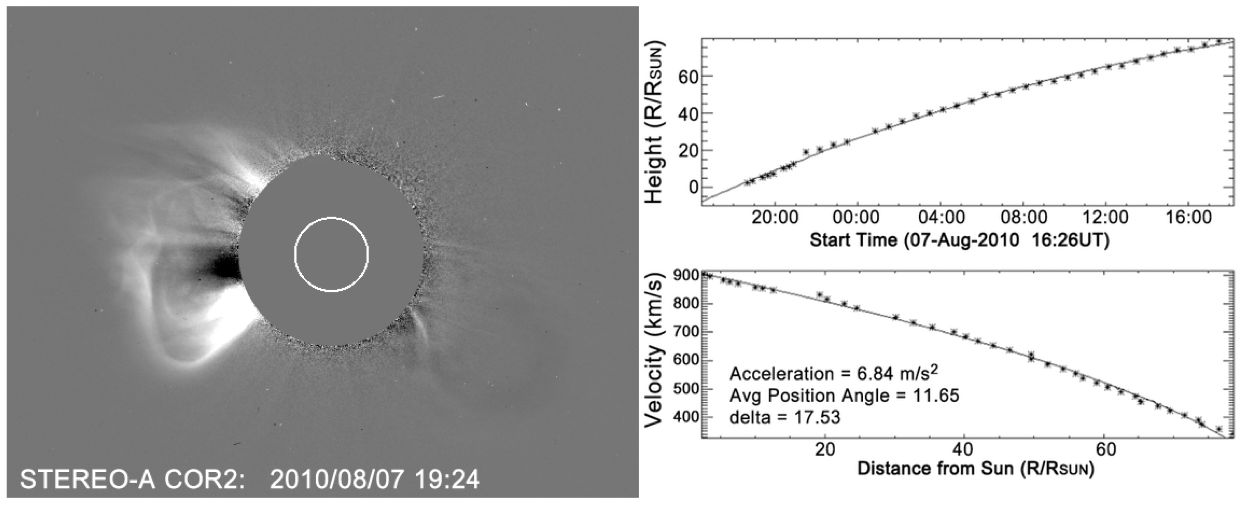
\includegraphics[width=150mm]{Images/Stereo2010Aug7Cme.png}
    \end{center}
    \label{stereo2010aug7}
\end{figure}

\paragraph{SDO/AIA EUV Image Observations}
The relative simplicity of this event is why it was chosen for a case study. The observations in AIA do not suggest that obscuration, waves, or Doppler shift contributed to the observed dimming. The area in the red contour of Figure \ref{aia2010aug7} was selected manually (by eye) to represent the region of mass loss, and its light curve shows clear dimming in 193 \AA\ and 171 \AA. In fact, the dimming from this region accounts for nearly all of the observed dimming throughout the entire event. This contour was selected after several iterations that indicated slight deviations in the contour had minimal impact on the light curve, as long as the dark region was fully encompassed. In other words, the result is fairly insensitive to the precise contour selection. The other contours were also selected manually to isolate regions of potential dimming e.g., as a sympathetic response from the solar eruptive event of interest. The exception is the magenta contour surrounding the flare loops that brightens dramatically but does not ever dim. 

\begin{figure}[!h]
	\caption[AIA contour analysis for 2010 August 7 event]{
        AIA results for the M1.0 Flare on 2010 August 7. Top: AIA 171 \AA\ channel difference image with subjectively 
        selected region contours overlaid. The red contour outlines what is thought to be the region of mass loss. The 
        orange and purple contours outline other active regions on the disk, which have the potential to have sympathetic 
        dimming. The green contour outlines a filament, which also has the potential to sympathetically dim based on its 
        behavior during the M flare on 2010 August 5. The magenta contour isolates the flaring coronal loops. The white line 
        around the solar limb is an artifact of the solarsoft derotation method. Bottom three plots: light curves of AIA 171 
        \AA, 193 \AA, and 304 \AA\ channels for the color-corresponding contours on the AIA image. The blue line is the 
        light curve for all on-disk area not enclosed by a contour. The black line is the sum of all contoured regions and 
        acts as a proxy for total dimming. All percent changes are calculated from the band’s value at 17:00 UT, prior to 
        the flare. The transition region He 304 \AA\ emission does not show dimming; both corona Fe emissions (171 \AA\ and 
        193 \AA) show dimming.
	}
    \begin{center}
	    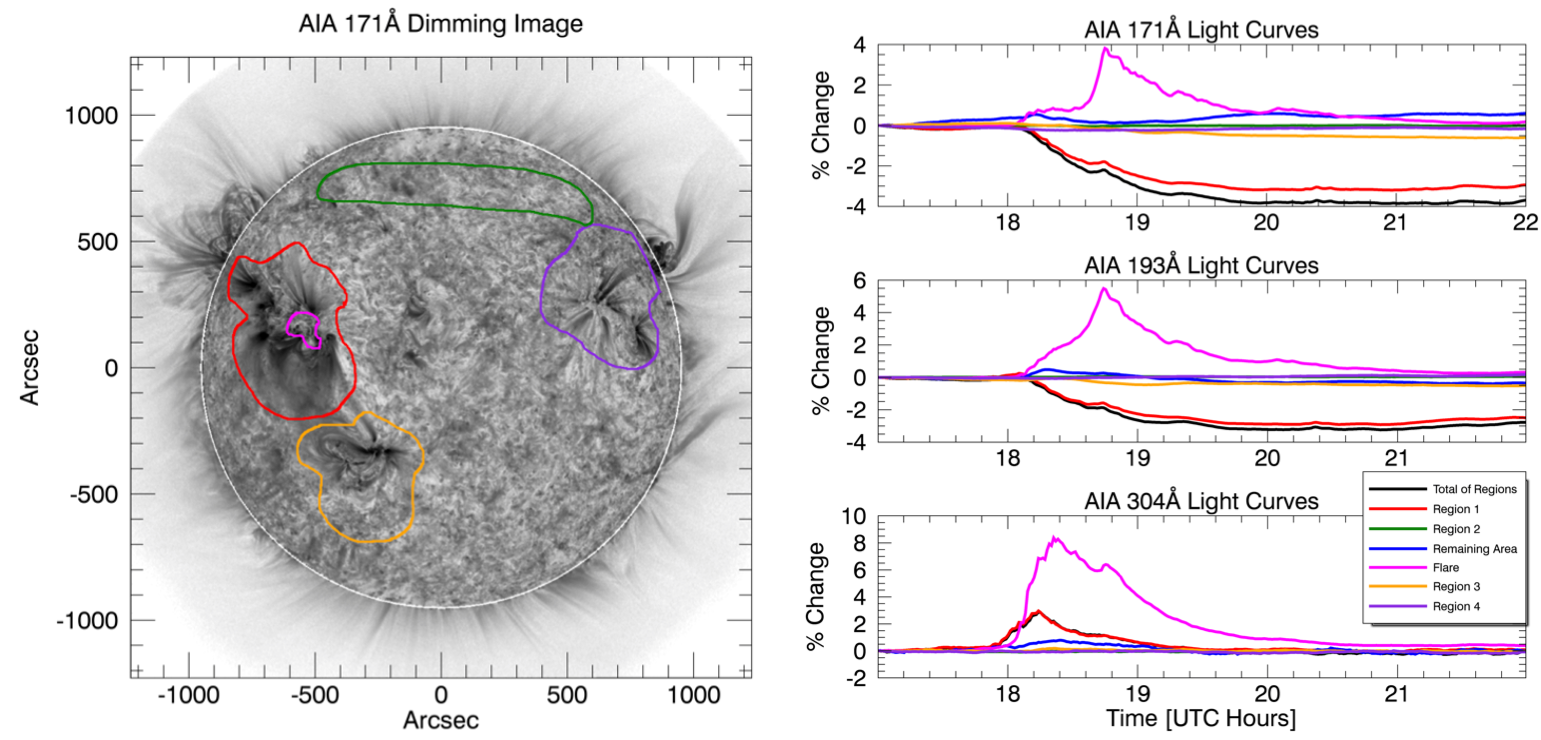
\includegraphics[width=166mm]{Images/Aia2010Aug7.png}
    \end{center}
    \label{aia2010aug7}
\end{figure}

The He II 304 \AA light curves are included to provide a contrast to the dimming effects seen in the coronal Fe lines. This He II wavelength is generated primarily in the chromosphere and transition region, as opposed to the coronal source of the other wavelengths. Mass loss occurs primarily in the corona, as the term coronal mass ejection suggests. This is reflected in the lack of dimming observed in the non-coronal He II 304 \AA\ emission line.

\begin{figure}[!h]
	\caption[AIA before/after images of 2010 August 7 event]{
	    AIA composite images (a) prior to solar eruptive event and (b) during deep dimming. In these images, purple is 
	    211 \AA, brownish-gold is 193 \AA, and yellow is 171 \AA. These static images show dimming in the region as outlined 
	    in Figure \ref{aia2010aug7}, though the change much more dramatic and obvious when viewed as a movie. 
	}
    \begin{center}
	    \includegraphics[width=166mm]{Images/AiaComposite2010Aug7.png}
    \end{center}
    \label{aiacomposite2010aug7}
\end{figure}

Thermal dimming may play a role in this event but may be difficult to quantify using only AIA because the relatively wide spectral bands of AIA channels mean many emission lines and any continua are blended together, which makes specifying a well-defined temperature difficult. Nevertheless, some indication of temperature is given by AIA and images that composite multiple wavelengths can aid in this analysis. Figure \ref{aiacomposite2010aug7} shows AIA composite images (211 \& 193 \& 171 \AA) before the solar eruptive event and during the dimming. All of these bands correspond primarily to the corona and transition region. If an area is dark, that means that there is little emission in all three of these wavelengths. Since these three bands span at least temperatures from 0.6-1.86 MK, that is indicative of mass loss. Even in areas of extreme heating, e.g., confined flare loops, it can be seen that emission is strong in all three of these bands resulting in the composite being white. Thus, it's unlikely that a region in these composite would become dark purely from a temperature change. EVE is less sensitive than AIA to blending in temperature space due to its higher spectral resolution and plethora of emission lines from Fe at different ionization states. A future study using the differential emission measure techniques of \citet{Caspi2014} to study the temperature evolution could help to quantify this effect.

\paragraph{SDO/EVE EUV Irradiance Observations}

\begin{figure}[!h]
	\caption[EVE selected emission lines for 2010 August 7 event]{
        One minute average EVE light curves of the 2010 August 7 coronal dimming event for the spectral lines listed in 
        Table <TODO: INSERT>, as well as the GOES 1–8 \AA\ channel light curve. The leftmost vertical dashed line indicates
        the GOES event start time, while the other vertical dashed line indicates the GOES event peak time. Peak formation 
        temperature of the EVE spectral lines increases from top to bottom plot. Fe IX to Fe XIII show clear dimming, Fe XIV
        is borderline, and Fe XV to Fe XX show smooth brightening with no dimming. The Fe XX 131 \AA\ profile is very 
        similar to GOES 1–8 \AA, indicating that this line in EVE is a good proxy for gradual phase timing. Also note the 
        vertical axes: dimming is on the order of a few percent for the cooler Fe emissions while the hotter Fe emissions 
        have bright peaks in the hundreds of percent. All percent changes are calculated from the spectral irradiance at 
        17:00 UT.
	}
    \begin{center}
	    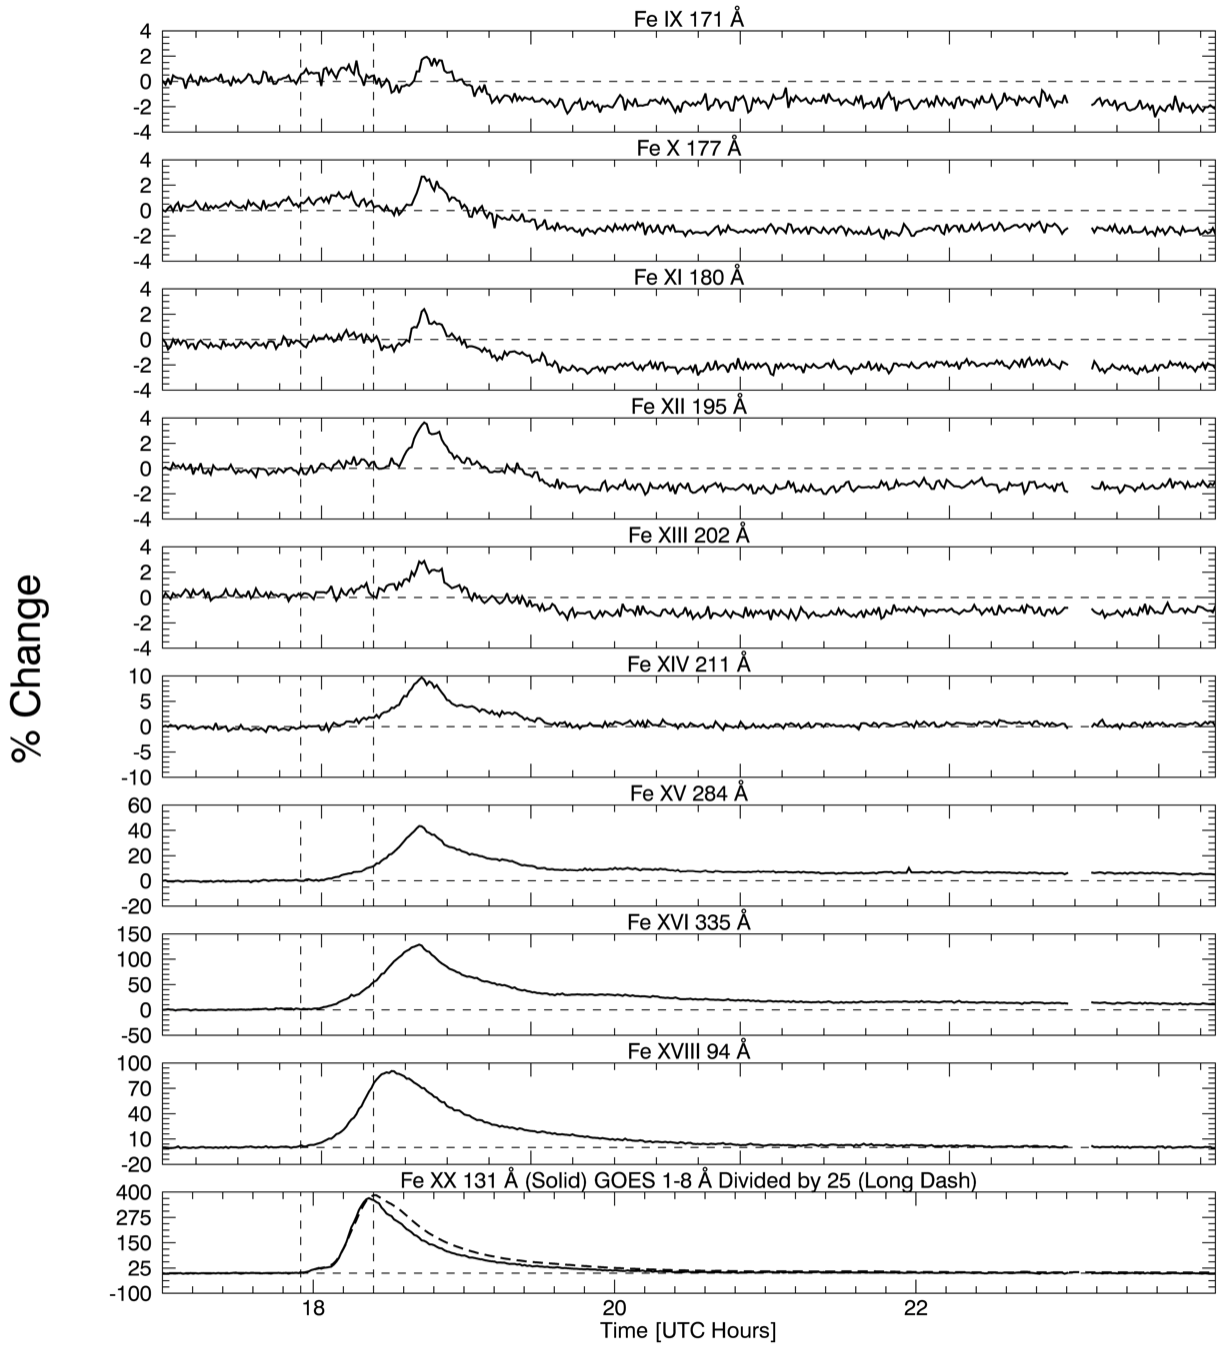
\includegraphics[width=166mm]{Images/Eve2010Aug7.png}
    \end{center}
    \label{eve2010aug7}
\end{figure}
Figure \ref{eve2010aug7} shows a trend that is consistent with the findings from Figure \ref{detectedDimmingVsIonization} -—that an ion’s peak formation temperature is inversely proportional to magnitude of dimming. The transition from an ionization state that shows dimming to ones that only show brightening occurs at Fe XIV 211 \AA, which itself shows dimming in some events but not others. The transition for where the Fe emission shows dimming is different for different solar eruptive events. For example, the Fe XVI 335 \AA\ emission has shown dimming for larger CME events \citep{Woods2011}. Herein, we will refer to Fe IX 171 \AA\ through Fe XIV 211 \AA\ as dimming lines for the 2010 August 7 event, and Fe XIV 211 \AA\ through Fe XXIV 192 \AA\ as nondimming lines (note that 211 \AA\ is included in both descriptions to reflect its ambiguity).

It is also interesting to note in Figure \ref{eve2010aug7} that the onset of dimming in the dimming lines is nearly simultaneous. The gradual-phase flare peak is delayed in lower ionizations of Fe, which is due to a cooling effect. The primary source of energy release in a flare is near the point of magnetic reconnection, typically far above the footpoints of the magnetic loops involved, in the corona. Some of the energy goes into the acceleration of particles downward. When these particles impact the denser chromosphere, they cause the heating and chromospheric evaporation. As that thermal plasma enters the corona it cools \citep{Fletcher2011}, and highly ionized Fe gains electrons. Thus, the peak is later for lower ionization states as seen in Figure \ref{eve2010aug7}. The Fe IX 171 \AA\ irradiance, in particular, shows the competing effects of this gradual phase flare peak and coronal dimming. Images with spatial resolution can isolate the flaring region responsible for this peak, as is shown with the magenta contour in Figure \ref{aia2010aug7}. Alternatively, we have developed a method for isolating and removing this peak in dimming lines with the spatially-integrated irradiance from EVE, which will be detailed in Section \ref{sec:deconvolve}. 

\subsection{Complex Dimming Case}
This event occurred on 2011 August 4 at approximately 3:47 UT. It spawned from NOAA active region 11261 at location N19W36. The eruptive event consisted of an M9.3 flare, a large and fast CME, and nearly all of the types of dimming discussed in Chapter \ref{chaptermechanisms}: mass-loss and thermal dimming, a global wave that then triggered a sympathetic filament eruption, an obscuration dimming from the filament. This event was chosen specifically for presenting so many types of dimming and related physical processes in a single case. 

\paragraph{Coronagraph Observations}
The CDAW catalog for this event lists it as a halo CME with a velocity of 1315 $km\ s^{-1}$, relatively fast for a CME, and a mass of $1.16 \times 10^{16}\ g$. However, halo CMEs present a strong challenge for obtaining accurate mass, and the catalog flags it as a poor mass estimate. Unfortunately, true-space velocity and mass have not been computed for this event using simultaneous quadrature observations from STEREO. Nevertheless, images from the three coronagraphs are shown in Figure . 

\begin{figure}[!h]
	\caption[LASCO and STEREO coronagraph data for 2011 August 4 event]{
        CME event associated with 2011 August 4 dimming event. From left to right the coronagraphs are STEREO Behind C2, 
        LASCO C3, and STEREO Ahead C2. Top: Snapshots prior to CME. Bottom: Snapshots during CME. 
    }
    \begin{center}
	    \includegraphics[width=166mm]{Images/Coronagraphs2011Aug4.png}
    \end{center}
    \label{coronagraphs2011aug4}
\end{figure}

\section{Flare-dimming Deconvolution Method}
\label{sec:deconvolve}

\section{Error Propagation}
\label{sec:deconvolveerrors}

\section{Dimming and CME Parameterization Results}
\label{sec:casestudyresults}

\subsection{Simple Dimming Case}

\subsection{Complex Dimming Case}

\section{Summary}
